%% ---------------------------------------------------------------------
%%  FIGURA - Curva do modelo de velocidade e pontos medidos (DG-11)
%%
%%  ATENCAO METODOLOGICA: a curva e o MODELO definido na especificacao
%%  (Equacao da secao 6.8). Os dois pontos sao MEDICOES da secao 8.5.
%%  Modelo e medicao nunca sao misturados nesta figura.
%% ---------------------------------------------------------------------
\begin{figure}[htb]
	\caption{Curva do modelo de velocidade da especificação e os dois valores medidos}
	\label{fig:velocidade}
	\centering
	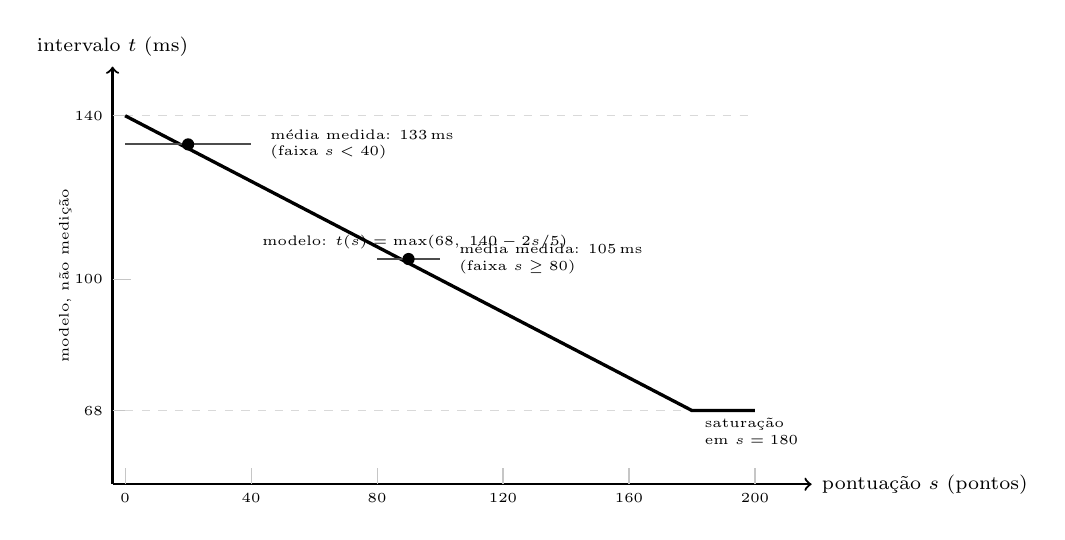
\begin{tikzpicture}[
			font=\scriptsize,
			x=0.040cm,
			y=0.052cm
		]

		% ---- eixos -----------------------------------------------------
		\draw[->, thick] (-4,50) -- (218,50) node[right] {pontuação $s$ (pontos)};
		\draw[->, thick] (-4,50) -- (-4,152) node[above, align=center] {intervalo $t$ (ms)};

		% ---- grade e marcas -------------------------------------------
		\foreach \x in {0,40,80,120,160,200} {
				\draw[gray!45, thin] (\x,50) -- (\x,54);
				\node[below, font=\tiny] at (\x,50) {\x};
			}
		\foreach \y in {68,100,140} {
				\draw[gray!45, thin] (-4,\y) -- (2,\y);
				\node[left, font=\tiny] at (-4,\y) {\y};
			}
		\draw[gray!30, dashed, thin] (0,68) -- (200,68);
		\draw[gray!30, dashed, thin] (0,140) -- (200,140);

		% ---- curva do modelo t(s) = max(68, 140 - 2s/5) ---------------
		\draw[very thick] (0,140) -- (180,68) -- (200,68);
		\node[above, font=\tiny, align=center] at (92,105) {modelo: $t(s) = \max(68,\; 140 - 2s/5)$};
		\node[right, font=\tiny, align=left] at (181,63) {saturação\\ em $s = 180$};

		% ---- faixas medidas ------------------------------------------
		% faixa baixa: pontuacao < 40, media medida 133 ms
		\draw[thick, black!70] (0,133) -- (40,133);
		\fill[black] (20,133) circle (2.2pt);
		\node[right, font=\tiny, align=left] at (43,133) {média medida: 133\,ms\\(faixa $s < 40$)};

		% faixa alta: pontuacao >= 80, media medida 105 ms
		\draw[thick, black!70] (80,105) -- (100,105);
		\fill[black] (90,105) circle (2.2pt);
		\node[right, font=\tiny, align=left] at (103,105) {média medida: 105\,ms\\(faixa $s \geq 80$)};

		% ---- anotacao do eixo y --------------------------------------
		\node[rotate=90, anchor=south, font=\tiny] at (-14,101) {modelo, não medição};
	\end{tikzpicture}
	\legend{Fonte: elaborado pelo autor (2026). A \textbf{curva} é o modelo declarado na especificação
	(Equação~(\ref{eq:velocidade-simplificada})), não uma medição. As \textbf{barras horizontais} são as
	faixas de pontuação sobre as quais cada média foi calculada, e os \textbf{círculos} são as médias
	medidas na Seção~\ref{sec:res-velocidade}. Os valores medidos incluem atraso positivo do ciclo de
	observação e não devem ser lidos como estimativas do parâmetro \texttt{stepMs}.}
\end{figure}
